\documentclass[dvipdfmx,11pt]{beamer}

\usepackage[deluxe]{otf} 
\usepackage{txfonts}
\renewcommand{\kanjifamilydefault}{\gtdefault}
\usepackage{amssymb,amsmath}
\usepackage{hyperref}
\usepackage[absolute,overlay]{textpos}
\usepackage{comment}
\usepackage{colortbl}
\usepackage{graphicx}
\usepackage{tikz}
\usetikzlibrary{positioning}
\usetikzlibrary{shadows}
\usepackage{listings}
\usepackage{plistings}
\usepackage{multicol}
\usepackage{multirow}
\def\lstlistingname{コード}
\newcommand{\code}[1]{\lstinline[basicstyle=\ttfamily]{#1}}
\newcommand{\lw}[1]{\smash{\lower-5.ex\hbox{#1}}}
\newcommand{\redunderline}[1]{\textcolor{red}{\underline{\textcolor{black}{#1}}}}

%%\usetheme{Frankfurt}
\usetheme{Warsaw}
\setbeamertemplate{navigation symbols}{} %スライドのボタン?(右下のやつ)を消す
\setbeamersize{text margin left=1.5em,text margin right=1.5em} % 余白なくすやつ

% footer setting %
\makeatother
\setbeamertemplate{footline}
{
  \leavevmode%
  \hbox{%
  \begin{beamercolorbox}[wd=.4\paperwidth,ht=2.25ex,dp=1ex,center]{author in head/foot}%
    \usebeamerfont{author in head/foot}\insertshortauthor
  \end{beamercolorbox}%
  \begin{beamercolorbox}[wd=.6\paperwidth,ht=2.25ex,dp=1ex,center]{title in head/foot}%
    \usebeamerfont{title in head/foot}\hspace*{1ex} \insertshorttitle\hspace*{3em}
    \textbf{ \insertframenumber{} / \inserttotalframenumber } \hspace*{1ex}
  \end{beamercolorbox}}%
  \vskip0pt%
}
\makeatletter

% exclude apprendix slides from framenumber %
\newcommand{\backupbegin}{
   \newcounter{framenumberappendix}
   \setcounter{framenumberappendix}{\value{framenumber}}
}
\newcommand{\backupend}{
   \addtocounter{framenumberappendix}{-\value{framenumber}}
   \addtocounter{framenumber}{\value{framenumberappendix}} 
}

\lstset{
 basicstyle=\ttfamily\color{black},
 keepspaces=true,
 escapechar=|,
 columns=[l]{fullflexible},
 commentstyle={\color{red}},
 stringstyle={\color{blue}}}

\title{解集合プログラミングを用いた\\配電網問題の解法に関する考察}
\author[山田 健太郎]{山田 健太郎}
\date{2020年度 番原研中間発表会 \\2020年12月11日}
\institute{番原研究室}

%#################################################
%# 本文 ##########################################
%#################################################
\begin{document}

%%%%%%%%%%%%%%%%%%%%%%%%%%%%%%%%%%%%%%%%%%%%%%%%%%
%% タイトル 
%%%%%%%%%%%%%%%%%%%%%%%%%%%%%%%%%%%%%%%%%%%%%%%%%%
\begin{frame}{}
  \titlepage
\end{frame}

%%%%%%%%%%%%%%%%%%%%%%%%%%%%%%%%%%%%%%%%%%%%%%%%%%
% 配電網
%%%%%%%%%%%%%%%%%%%%%%%%%%%%%%%%%%%%%%%%%%%%%%%%%%
\begin{frame}{配電網問題}
  \begin{alertblock}{}\centering
    求解困難な組合せ最適化問題の一種
  \end{alertblock}
  \vfill
  \begin{itemize}
  \item \alert{\bf 配電網}とは,変電所と,一般家庭や工場を繋ぐ電力供給
    経路のネットワークである.
  \item  配電網の構成技術はスマートグリッドや,災害時の障害箇所の迂回
    構成などを支える重要な基盤技術として期待されている.
  \item \alert{\bf 配電網問題}とは,
    \begin{itemize}
    \item \structure{\bf トポロジ制約}と\structure{\bf 電気制約}を満たしつつ,
    \item 損失電力を最小にするスイッチの開閉状態を求めることが目的.
    \end{itemize}
  \item これまで,メタヒューリスティクス等の解法が提案されている.
  \item 厳密解法としては,フロンティア法を用いた解法が提案されており
    \begin{itemize}
    \item 実用規模の配電網問題(\structure{\textbf{スイッチ数468個}})の
      最適解を求めることに成功~[井上ほか '12].
    \end{itemize}
  \end{itemize}
\end{frame}

% %%%%%%%%%%%%%%%%%%%%%%%%%%%%%%%%%%%%%%%%%%%%%%%%%%
% %% ASP
% %%%%%%%%%%%%%%%%%%%%%%%%%%%%%%%%%%%%%%%%%%%%%%%%%%
% \begin{frame}{解集合プログラミング(Answer Set Programming; ASP)}
%   \begin{itemize}
%   \item \structure{\bf ASPの言語}は一階論理に基づく知識表現言語の一種である.
%   \item \structure{\bf ASPシステム}は論理プログラムから安定モデル意味
%     論~[Gelfond and Lifschitz '88]に基づく解集合を計算するシステムである.
%   \item 近年,SATソルバーの実装技術を応用した高速ASPシステムが実現され,
%     システム検証,プランニング,システム生物学など様々な分野への応用が
%     拡大している.
%   \end{itemize}
%   \vfill
%   \begin{alertblock}{配電網問題に対してASP技術を用いる利点}
%     \begin{itemize}
%     \item ASP言語の高い表現力を生かし,各種制約を\textbf{簡潔に記述可能}
%     \item マルチショットASP解法により,
%       ある配電網構成(スタート状態)から他の配電網構成(ゴール状態)
%       へのスイッチの切替手順を求める\textbf{遷移問題への拡張が容易}
%     \item 背景理論つきASPにより,様々な\textbf{背景理論ソルバーと連携可能}
%     \item 解の最適性を保証でき,最適解の列挙も可能
%     \end{itemize}
%   \end{alertblock}
% \end{frame}

%%%%%%%%%%%%%%%%%%%%%%%%%%%%%%%%%%%%%%%%%%%%%%%%%% 
%% 根付き全域森
%%%%%%%%%%%%%%%%%%%%%%%%%%%%%%%%%%%%%%%%%%%%%%%%%%
\begin{frame}{トポロジ制約}
  \begin{alertblock}{}
    トポロジ制約のみの配電網問題は,グラフと根と呼ばれる特別なノードから,
    \alert{\bf 根付き全域森}を求める部分グラフ探索問題に帰着できる.
  \end{alertblock}
  \vfill
  \begin{block}{根付き全域森 (Spanning Rooted Forest) [川原・湊 '12]}
    グラフ$G=(V,E)$と,
    \textbf{根}と呼ばれる$V$上のノードが与えられたとき,
    $G$上の根付き全域森とは,以下の条件を満たす$G$の部分グラフ$G'=(V,E'),\ E' \subseteq E$である.
    \begin{enumerate}
    \item $G'$はサイクルを持たない. (\alert{\bf 非閉路制約})
    \item $G'$の各連結成分は,ちょうど1つの根を含む. (\alert{\bf 根付き連結制約})
    \end{enumerate}
  \end{block}\vfill
 \begin{itemize}
  \item この部分グラフ探索問題を\structure{\bf 根付き全域森問題}と呼ぶ.
 \end{itemize}
\end{frame}
%%%%%%%%%%%%%%%%%%%%%%%%%%%%%%%%%%%%%%%%%%%%%%%%%%
%% 根付き全域森の例
%%%%%%%%%%%%%%%%%%%%%%%%%%%%%%%%%%%%%%%%%%%%%%%%%%
\begin{frame}{根付き全域森問題の例}
  \begin{columns}
    \begin{column}{0.45\textwidth}\centering
      \begin{exampleblock}{入力例}
	\centering
	%%%%%%%%%%%%%%%%%%%%%%%%%%%%%%%%%%%%%%%%%%%%%%%%%%
% 根付き全域森の例
%%%%%%%%%%%%%%%%%%%%%%%%%%%%%%%%%%%%%%%%%%%%%%%%%%

\begin{tikzpicture}[scale=0.5]

 % 設定
 \tikzset{node/.style={circle,draw=black,fill=white}}

 \definecolor{edge1}{RGB}{191,0,0}
 \definecolor{node1}{RGB}{249,200,200}
 \definecolor{edge3}{RGB}{38,38,134}
 \definecolor{node3}{RGB}{200,200,249}

 % 補助線
 % \draw [help lines,blue] (0,0) grid (20,6);

 % 入力されるグラフ
 % node %
 \node[circle, ultra thick,draw=edge1,fill=node1] (in1) {1};
 \node[node,right= of in1] (in2){2};
 \node[circle, ultra thick, draw=edge3,fill=node3, right=of in2](in3){3};
 \node[node,below= of in1] (in4){4};
 \node[node,below= of in2] (in5){5};
 \node[node,below= of in3] (in6){6};

 % 辺
 \foreach \u / \v in {in1/in2,in2/in3,in1/in4,in2/in5,in3/in6,in4/in5,in5/in6}
 \draw (\u) -- (\v);

\end{tikzpicture}

%%%%%%%%%%%%%%%%%%%%%%%%%%%%%%%%%%%%%%%%%%%%%%%%%%%%%%%%%%
%%% Local Variables:
%%% mode: japanese-latex
%%% TeX-master: ``slide''
%%% End:

      \end{exampleblock}
    \end{column}
    \begin{column}{0.05\textwidth}\centering
      $\Rightarrow$
    \end{column}
    \begin{column}{0.45\textwidth}\centering
      \begin{exampleblock}{解の例}
        \centering
        %%%%%%%%%%%%%%%%%%%%%%%%%%%%%%%%%%%%%%%%%%%%%%%%%%
% 根付き全域森の例
%%%%%%%%%%%%%%%%%%%%%%%%%%%%%%%%%%%%%%%%%%%%%%%%%%

\begin{tikzpicture}[scale=0.5]

 % 設定
 \tikzset{node/.style={circle,draw=black,fill=white}}

 \definecolor{edge1}{RGB}{191,0,0}
 \definecolor{node1}{RGB}{249,200,200}
 \definecolor{edge3}{RGB}{38,38,134}
 \definecolor{node3}{RGB}{200,200,249}

 % 補助線
 % \draw [help lines,blue] (0,0) grid (20,6);

 % node %
 \node[circle, ultra thick, draw=edge1, fill=node1](out1){1};
 \node[node, fill=node1, right=of out1] (out2){2};
 \node[circle, ultra thick, draw=edge3,fill=node3, right=of out2](out3){3};
 \node[node, fill=node1, below=of out1] (out4){4};
 \node[node, fill=node3, below=of out2] (out5){5};
 \node[node, fill=node3, below=of out3] (out6){6};

 \foreach \u / \v in {out1/out2,out1/out4}
 \draw [very thick, edge1] (\u) -- (\v);

 \foreach \u / \v in {out3/out6,out5/out6}
 \draw [very thick, edge3](\u) -- (\v);

\end{tikzpicture}

%%%%%%%%%%%%%%%%%%%%%%%%%%%%%%%%%%%%%%%%%%%%%%%%%%%%%%%%%%
%%% Local Variables:
%%% mode: japanese-latex
%%% TeX-master: ``slide''
%%% End:

      \end{exampleblock}
    \end{column}
  \end{columns}
  \vfill
  \begin{itemize}
  \item \structure{\bf 配電網とグラフの対応} \\
	 \begin{center}
      \begin{minipage}[c]{0.6\textwidth}
	   \begin{block}{}
		\centering
		\begin{tabular}{c|ccc}
		配電網 & 配電区間 & スイッチ & 変電所 \\
		\hline
		グラフ & ノード & 辺 & 根
		\end{tabular}
	   \end{block}
      \end{minipage}
	 \end{center}\vfill
   \item \structure{\bf 配電網問題のトポロジ制約}
		 \begin{itemize}
		  \item 停電(変電所と結ばれない区間)
		  \item 短絡(供給経路上のループ,複数の変電所と結ばれる区間)
		 \end{itemize}
  \end{itemize}
\end{frame}
%%%%%%%%%%%%%%%%%%%%%%%%%%%%%%%%%%%%%%%%%%%%%%%%%%
%% 電気制約
%%%%%%%%%%%%%%%%%%%%%%%%%%%%%%%%%%%%%%%%%%%%%%%%%%
\begin{frame}{電気制約}
 \begin{itemize}
  \item \structure{\bf 電気制約}は,配電する\structure{\bf 電流・電圧}の適正範囲を保証する制約.
  \item 電流が許容範囲を超えてしまうと,配電線が焼き切れてしまい,停電や事故などの危険につながってしまう.
  \item 電圧が許容範囲を下回ってしまうと,配電先で機械や電化製品が適切に動作できないなどの
		問題が発生してしまう.
  \item 配電システムによっては,その他にも様々な制約がある.
 \end{itemize}
 \vfill
 \begin{alertblock}{ASPを用いて実装する上での課題}
  \begin{itemize}
   \item 電流や電圧が影響し合う実数ドメイン上の制約である.
   \item 虚数を含むインピーダンスの計算など,純粋なASPのみで扱うには難しいと考えられる.
  \end{itemize}
 \end{alertblock}\vfill
\end{frame}

%%%%%%%%%%%%%%%%%%%%%%%%%%%%%%%%%%%%%%%%%%%%%%%%%%
%% 研究目的
%%%%%%%%%%%%%%%%%%%%%%%%%%%%%%%%%%%%%%%%%%%%%%%%%%
\begin{frame}{研究目的}
  \begin{alertblock}{目的}\centering
    ASP技術を活用して,大規模な配電網問題を効率良く解くシステムを構築
    する.
  \end{alertblock}
  \vfill
  \begin{block}{研究内容}
    \begin{enumerate}
    \item \structure{\bf 根付き全域森問題を解くASP符号化を新たに1種類考案}
      \begin{itemize}
	   \item 有向グラフの次数を用いた符号化
      \end{itemize}
	 \item \structure{\bf 実用規模の問題,および,より大規模な問題を用いて評価}
	 \item \structure{\bf 電気制約の実装への方針}
      \begin{itemize}
	   \item 電流に関する電気制約
      \end{itemize}
    \end{enumerate}
  \end{block}
\end{frame}
%%%%%%%%%%%%%%%%%%%%%%%%%%%%%%%%%%%%%%%%%%%%%%%%%%
%% 提案手法
%%%%%%%%%%%%%%%%%%%%%%%%%%%%%%%%%%%%%%%%%%%%%%%%%%
\begin{frame}\frametitle{提案するASP符号化}
 
\begin{itemize}
 \item  根付き全域森問題のASP符号化を新たに1つ考案した.
% \item $|V|$はグラフのノード数,$|R|$は根ノード数をそれぞれ表す.
\end{itemize}
 
\begin{table}[t]
 \centering
 %%%%%%%%%%%%%%%%%%%%%%%%%%%%%%%%%%%%%%%%%%%%%%%%%%%%%%%%%%%%%%%%
\chapter{ハミルトン閉路問題および関連問題のASP符号化}\label{chap:proposal}
%%%%%%%%%%%%%%%%%%%%%%%%%%%%%%%%%%%%%%%%%%%%%%%%%%%%%%%%%%%%%%%% 

%%%%
\begin{figure}[h]
  \centering
  \thicklines
  \setlength{\unitlength}{1.2pt}
  \small\footnotesize\scriptsize
  \begin{picture}(280,57)(4,-10)
    \put(  0, 20){\dashbox(50,24){\shortstack{HCP問題\\インスタンス}}}
    \put( 60, 20){\framebox(50,24){変換器}}
    \put(120, 20){\dashbox(50,24){\shortstack{ASPファクト}}}
    \put(120,-10){\dashbox(50,24){\shortstack{ASP符号化\\(論理プログラム)}}}
    \put(180, 20){\framebox(50,24){ASPシステム}}
    \put(240, 20){\dashbox(50,24){\shortstack{HCP問題\\の解}}}
    \put( 50, 32){\vector(1,0){10}}
    \put(110, 32){\vector(1,0){10}}
    \put(170, 32){\vector(1,0){10}}
    \put(230, 32){\vector(1,0){10}}
    \put(170, +2){\line(1,0){4}}
    \put(174, +2){\line(0,1){30}}
  \end{picture}  
\caption{ASP を用いたハミルトン閉路問題(HCP)の解法}
\label{fig:arch}
\end{figure}
%%%%

%\begin{figure}[tbp]
\tikz{
  %1ノード目
  \path[draw=black, fill=blue!20, rounded corners=5pt]%線の設定
  node[at={(0.75,0.75)}] {問題}%文字を入れる
  (0,0) --(1.5,0) --(1.5,1.5) --(0,1.5) --cycle;%外周
  %2ノード目
  \path[draw=black, fill=blue!20, rounded corners=5pt, shift={(3,0)}]
  node[at={(0.75,0.75)}] {
    \begin{tabular}{c}
      ASP\\
      ファクト
    \end{tabular}
  }
  (0,0) --(1.5,0) --(1.5,1.5) --(0,1.5) --cycle;
  %3ノード目文字が複数行
  \path[draw=black, fill=green!20, rounded corners=5pt, shift={(6,0)}]
  node[at={(0.75,0.75)}] {
    \begin{tabular}{c}
      ASP\\
      システム
    \end{tabular}
  }
  (0,0) --(1.5,0) --(1.5,1.5) --(0,1.5) --cycle;
  %4ノード目文字が複数行
  \path[draw=black, fill=blue!20, rounded corners=5pt, shift={(9,0)}]
  node[at={(0.75,0.75)}] {解集合}
  (0,0) --(1.5,0) --(1.5,1.5) --(0,1.5) --cycle;
  %5ノード目文字が複数行
  \path[draw=black, fill=red!20, rounded corners=5pt, shift={(3,-3)}]
  node[at={(0.75,0.75)}] {
    \begin{tabular}{c}
      ASP\\
      符号化
    \end{tabular}
  }
  (0,0) --(1.5,0) --(1.5,1.5) --(0,1.5) --cycle;
  \draw[arrows=->] (1.5,0.75) --(3.0,0.75);
  \draw[arrows=->,shift={(3,0)}] (1.5,0.75) --(3.0,0.75);
  \draw[arrows=->,shift={(6,0)}] (1.5,0.75) --(3.0,0.75);
  \draw[arrows=->] (4.5,-2.25) --(6.0,0.5);
}
\caption{ASPを用いた解法}
\label{aspmethod}
\end{figure}


ASP を用いたハミルトン閉路問題および関連問題の解法について述べる.
図~\ref{fig:arch}に,解法の流れを示す.
与えられたハミルトン閉路問題は ASP ファクトに変換され,
ハミルトン閉路問題を解く ASP 符号化と結合され,
ASP システムによって解が計算される.
本論文では,ASP システムとして{\clingo}を用いる.

%%%%%%%%%%%%%%%%%%%%%%%%%%%%%%%%%%%%%%%%%%%%%%%%%%%%%%%%%%%%%%%%%%%%%%%
\section{ASPファクト形式}
%%%%%%%%%%%%%%%%%%%%%%%%%%%%%%%%%%%%%%%%%%%%%%%%%%%%%%%%%%%%%%%%%%%%%%%

%%%%%%%%%%%%%%%%%%%%%%%%%%%%%%
\begin{figure}[t]
\begin{center}
\begin{tikzpicture}
  %ノード1  
  \draw(4,2) circle (0.5)
  node[at={(4.1,2.1)}] {
    \begin{tabular}{c}
      1
    \end{tabular}
  };
  %ノード2  
  \draw(4,0) circle (0.5)
  node[at={(4.1,0.1)}] {
    \begin{tabular}{c}
      2
    \end{tabular}
  };
  %ノード3  
  \draw(6,2) circle (0.5)
  node[at={(6.1,2.1)}] {
    \begin{tabular}{c}
      3
    \end{tabular}
  };
  %ノード4  
  \draw(6,0) circle (0.5)
  node[at={(6.1,0.1)}] {
    \begin{tabular}{c}
      4
    \end{tabular}
  };
  %ノード5  
  \draw(8,2) circle (0.5)
  node[at={(8.1,2.1)}] {
    \begin{tabular}{c}
      5
    \end{tabular}
  };
  %ノード6  
  \draw(8,0) circle (0.5)
  node[at={(8.1,0.1)}] {
    \begin{tabular}{c}
      6
    \end{tabular}
  };
\draw(4,0.5) --(4,1.5);
\draw(6,0.5) --(6,1.5);
\draw(8,0.5) --(8,1.5);
\draw(4.5,0) --(5.5,0);
\draw(4.5,2) --(5.5,2);
\draw(6.5,0) --(7.5,0);
\draw(6.5,2) --(7.5,2);
\end{tikzpicture}

\caption{入力となる重み付き無向グラフの例}
\label{graphexample}
\end{center}
\end{figure}
%%%%%%%%%%%%%%%%%%%%%%%%%%%%%%

%%%%%%%%%%%%%%%%%%%%%%%%%%%%%%
\lstinputlisting[float=t,caption={%
図~\ref{graphexample}のASPファクト表現},%
captionpos=b,frame=single,label=code:graph_example.lp,%
numbers=none,%
breaklines=true,%
columns=fullflexible,keepspaces=true,%
basicstyle=\ttfamily\scriptsize]{code/graph_example.lp}
%%%%%%%%%%%%%%%%%%%%%%%%%%%%%%


本節では,最短ハミルトン閉路問題の例にとって,
入力となる重み付き無向グラフ(図~\ref{graphexample})の
ASP ファクト形式について説明する.
%
このグラフは,頂点数が6,辺の数が7であり,辺に付けられた値は距離を表す.
コード~\ref{code:graph_example.lp}に,ASPファクト形式を示す.
%
アトム\code{node/1}は頂点,\code{edge/2}は辺,\code{cost/3}は距離を表す.
例えば,\code{cost(1,2,3)}は,辺\code{edge(1,2)}の距離が3であることを
表している.

%%%%%%%%%%%%%%%%%%%%%%%%%%%%%%%%%%%%%%%%%%%%%%%%%%%%%%%%%%%%%%%%%%%%%%%
\section{ハミルトン閉路問題の ASP 符号化}\label{hamiltonianasp}
%%%%%%%%%%%%%%%%%%%%%%%%%%%%%%%%%%%%%%%%%%%%%%%%%%%%%%%%%%%%%%%%%%%%%%%

ハミルトン閉路問題は,与えられたグラフの全頂点をちょうど一度ずつ通る閉
路(ハミルトン閉路)が存在するかどうかを判定する問題である.
$G=(V,E)$にハミルトン閉路が存在する必要十分条件は,
以下の2つの制約を満たす部分グラフ$G'=(V,E')$が存在することである.

\begin{itemize}
\item $G'$の各頂点の次数が2 (次数制約)
\item $G'$が連結である (連結制約)
\end{itemize}

本論文では,前者を\textbf{次数制約},後者を\textbf{連結制約}と呼ぶ.
ハミルトン路問題は,ハミルトン閉路問題から始点と終点が一致するという閉
路の条件を取り除いたものである.
ハミルトン路問題では,次数制約は以下のように変わる.

\begin{itemize}
\item 始点と終点の次数が1,他の頂点の次数が2
\end{itemize}

以下では,ハミルトン閉路問題に対する3つの ASP 符号化
\textsf{undirected},\textsf{directed},\textsf{acyclicity}
を提案する.

%%%%%%%%%%%%%%%%%%%%%%%%%%%%%%%%%%%%%%%%%%%%%%%%%%%%%%%%%%%%%%%%%%%%%%%
\subsection{\textsf{undirected}符号化}
%%%%%%%%%%%%%%%%%%%%%%%%%%%%%%%%%%%%%%%%%%%%%%%%%%%%%%%%%%%%%%%%%%%%%%%

%%%%%%%%%%%%%%%%%%%%%%%%%%%%%%
\lstinputlisting[float=t,caption={%
\textsf{undirected}符号化},%
captionpos=b,frame=single,label=code:hamilton1.lp,%
numbers=left,%
breaklines=true,%
columns=fullflexible,keepspaces=true,%
basicstyle=\ttfamily\footnotesize]{code/hamilton1.lp}
%%%%%%%%%%%%%%%%%%%%%%%%%%%%%%

\textsf{undirected}符号化は,ハミルトン閉路問題の次数制約と連結制約を,
ASP の一貫性制約で表した基本的な符号化である.
コード~\ref{code:hamilton1.lp}に,\textsf{undirected}符号化を示す.
この符号化は,ハミルトン閉路問題とハミルトン路問題の両方に対応している.
符号化中の\code{s}は始点の頂点番号,\code{t}は終点の頂点番号を表し,こ
れらは実行時に与えられる.
ここでは,ハミルトン閉路問題(\code{s}=\code{t})の場合について説明する.

\begin{itemize}
\item 1行目のルールは,各辺\code{edge(X,Y)}に対して,その辺がハミルト
  ン閉路に含まれるかどうかを意味するアトム\code{in(X,Y)}を選択子を用い
  て導入している.
\item 次数制約は3行目のルールで表される.このルールは,
  各頂点\code{node(X)}に対して,その次数の和が2に等しいことを個数制約
  を使って表している.
\item 連結制約は11行目のルールで表される.
ある頂点\code{X}が始点\code{s}から到達可能であることを意味する補助アト
ム\code{reached(X)}を導入する.
8行目のルールは,始点\code{s}が到達可能あることを表している.
9行目のルールは,各辺\code{X}--\code{Y}に対して,その辺がハミルトン閉
路に含まれ(\code{in(X,Y)}),かつ,頂点\code{X}が始点から到
達可能であれば(\code{reached(X)}),\code{Y}も到達可能であることを表している.
10行目は9行目と同様であるが,辺\code{Y}--\code{X}の場合を表している.
11行目のルールは,各頂点\code{node(X)}が始点から到達可能でなければな
らないことを一貫性制約を使って表している.
\end{itemize}

%%%%%%%%%%%%%%%%%%%%%%%%%%%%%%%%%%%%%%%%%%%%%%%%%%%%%%%%%%%%%%%%%%%%%%%
\subsection{\textsf{directed}符号化}
%%%%%%%%%%%%%%%%%%%%%%%%%%%%%%%%%%%%%%%%%%%%%%%%%%%%%%%%%%%%%%%%%%%%%%%

%%%%%%%%%%%%%%%%%%%%%%%%%%%%%%
\lstinputlisting[float=t,caption={%
\textsf{directed}符号化},%
captionpos=b,frame=single,label=code:hamilton2.lp,%
numbers=left,%
breaklines=true,%
columns=fullflexible,keepspaces=true,%
basicstyle=\ttfamily\footnotesize]{code/hamilton2.lp}
%%%%%%%%%%%%%%%%%%%%%%%%%%%%%%

\textsf{directed}符号化は,\textsf{undirected}符号化をベースに,
与えられた無向グラフの各辺$u-v$に対して,2つの弧$u\rightarrow v$と
$v\rightarrow u$を対応させることで有向グラフ化して解く符号化である.
コード~\ref{code:hamilton2.lp}に,\textsf{directed}符号化を示す.
前節と同様に,ハミルトン閉路問題(\code{s}=\code{t})の場合について説明する.

\begin{itemize}
\item 1行目では,無向グラフの有向グラフ化を行う.
  与えられた無向グラフの各辺\code{edge(X,Y)}に対して,
  2つの弧\code{edge(X,Y)},\code{edge(Y,X)}を導入した.
\item 2行目のルールは,各弧\code{edge(X,Y)}に対して,その弧がハミルト
  ン閉路に含まれるかどうかを意味するアトム\code{in(X,Y)}を選択子を用い
  て導入している.
\item 次数制約は4,5行目のルールで表される.
  4行目では,各頂点\code{node(X)}に対して,
  その出次数が1に等しいことを個数制約を使って表している.
  5行目では,入次数について4行目と同様の制約を表す.
\item 連結制約は15行目のルールで表される.
  ある頂点\code{X}が始点\code{s}から到達可能であることを意味する
  補助アトム\code{reached(X)}を導入する.
  13行目のルールは,始点\code{s}が到達可能あることを表している.
  14行目のルールは,各弧\code{X}--\code{Y}に対して,その弧がハミルトン閉路
  に含まれ(\code{in(X,Y)}),かつ,頂点\code{X}が始点から
  到達可能であれば(\code{reached(X)}),\code{Y}も到達可能であることを表している.
  15行目のルールは,各頂点\code{node(X)}が始点から到達可能でなければ
  ならないことを一貫性制約を使って表している.
\item 18行目のルールは,解についての対称性を除去する.
  与えられた無向グラフ上の各ハミルトン閉路に対して,
  それを変換した有向グラフ上のハミルトン閉路は対称な2つが存在する.
  これによる解の重複を防ぐために,18行目のルールは,各弧\code{s}--\code{X},
  \code{Y}--\code{s}がハミルトン閉路に含まれるならば(\code{in(s,X),in(Y,s)}),
  \code{X < Y}でなければならないことを,一貫性制約を用いて表している
\end{itemize}

%%%%%%%%%%%%%%%%%%%%%%%%%%%%%%%%%%%%%%%%%%%%%%%%%%%%%%%%%%%%%%%%%%%%%%%
\subsection{\textsf{acyclicity}符号化}
%%%%%%%%%%%%%%%%%%%%%%%%%%%%%%%%%%%%%%%%%%%%%%%%%%%%%%%%%%%%%%%%%%%%%%%

%%%%%%%%%%%%%%%%%%%%%%%%%%%%%%
\lstinputlisting[float=t,caption={%
\textsf{acyclicity}符号化},%
captionpos=b,frame=single,label=code:hamilton3.lp,%
numbers=left,%
breaklines=true,%
columns=fullflexible,keepspaces=true,%
basicstyle=\ttfamily\footnotesize]{code/hamilton3.lp}
%%%%%%%%%%%%%%%%%%%%%%%%%%%%%%

\textsf{acyclicity}符号化は,\textsf{directed}符号化をベースに,
連結の制約に代わる部分閉路禁止制約を組込み非閉路制約で表現した符号化である.
コード~\ref{code:hamilton3.lp}に,\textsf{acyclicity}符号化を示す.
前節と同様に,ハミルトン閉路問題(\code{s}=\code{t})の場合について説明する.

\begin{itemize}
\item 1行目では,無向グラフの有向グラフ化を行う.
  与えられた無向グラフの各辺\code{edge(X,Y)}に対して,
  2つの弧\code{edge(X,Y)},\code{edge(Y,X)}を導入した.
\item 2行目のルールは,各弧\code{edge(X,Y)}に対して,その弧がハミルト
  ン閉路に含まれるかどうかを意味するアトム\code{in(X,Y)}を選択子を用い
  て導入している.
\item 次数制約は4,5行目のルールで表される.
  4行目では,各頂点\code{node(X)}に対して,
  その出次数が1に等しいことを個数制約を使って表している.
  5行目では,入次数について4行目と同様の制約を表す.
\item 部分閉路禁止制約は14行目のルールで表される.
  このルールは,始点でない各頂点\code{X},\code{Y}について,
  弧\code{X}--\code{Y}がハミルトン閉路に含まれるならば(\code{in(X,Y)}),
  そのような弧の集合をもつグラフが閉路をもたないことを,\code{#edge}宣言を用いて表す.
  ようするに,始点(終点)を含まないような閉路を禁止している.
\item 17行目のルールは,解についての対称性を除去する.
  与えられた無向グラフ上の各ハミルトン閉路に対して,
  それを変換した有向グラフ上のハミルトン閉路は対称な2つが存在する.
  これによる解の重複を防ぐために,17行目のルールは,各弧\code{s}--\code{X},
  \code{Y}--\code{s}がハミルトン閉路に含まれるならば(\code{in(s,X),in(Y,s)}),
  \code{X < Y}でなければならないことを,一貫性制約を用いて表している
\end{itemize}

%%%%%%%%%%%%%%%%%%%%%%%%%%%%%%%%%%%%%%%%%%%%%%%%%%%%%%%%%%%%%%%%%%%%%%% 
\section{最短ハミルトン閉路問題のASP符号化}\label{minexpl}
%%%%%%%%%%%%%%%%%%%%%%%%%%%%%%%%%%%%%%%%%%%%%%%%%%%%%%%%%%%%%%%%%%%%%%% 

%% %%%%%%%%%%%%%%%%%%%%%%%%%%%%%%
%% \lstinputlisting[caption =  最適化,label = minimize]{code/obj_minimize.lp}
%% %%%%%%%%%%%%%%%%%%%%%%%%%%%%%%

%%%%%%%%%%%%%%%%%%%%%%%%%%%%%%
\lstinputlisting[float=t,caption={%
最小化},%
captionpos=b,frame=single,label=code:obj_minimize.lp,%
numbers=left,%
breaklines=true,%
columns=fullflexible,keepspaces=true,%
basicstyle=\ttfamily\footnotesize]{code/obj_minimize.lp}
%%%%%%%%%%%%%%%%%%%%%%%%%%%%%%

最短ハミルトン閉路問題の目的関数は,
ハミルトン閉路を構成する各辺の距離の総和である.
コード\ref{code:obj_minimize.lp}は,
その目的関数の最小化を表す.
このコードは,各辺\code{edge(X,Y)}に対して,その辺がハミルトン閉路に
含まれ(\code{in(X,Y)}),その距離が\code{C}である時に(\code{cost(X,Y,C)}),
\code{C}の総和の最小化を,最小化関数を用いて表している.
.
%%%%%%%%%%%%%%%%%%%%%%%%%%%%%%
\lstinputlisting[float=t,caption={%
重み付き無向グラフの有向グラフ化},%
captionpos=b,frame=single,label=code:cost_both.lp,%
numbers=left,%
breaklines=true,%
columns=fullflexible,keepspaces=true,%
basicstyle=\ttfamily\footnotesize]{code/cost_both.lp}
%%%%%%%%%%%%%%%%%%%%%%%%%%%%%%

符号化directed,acyclicityについては,
与えられた無向グラフの各辺\code{edge(X,Y)}に対して,
2つの弧\code{edge(X,Y)},\code{edge(Y,X)}を導入した.
各辺の距離もこれに対応させるために,コード\ref{code:cost_both.lp}
を追加した.
このルールは,各辺\code{X}--\code{Y}の距離を表す\code{cost(X,Y,C)}について,
\code{cost(Y,X,C)}を導入する.
これにより,与えられた無向グラフの各辺\code{edge(X,Y)}の重み\code{C}が
2つの弧\code{edge(X,Y)},\code{edge(Y,X)}にも付与された.

%%%%%%%%%%%%%%%%%%%%%%%%%%%%%%%%%%%%%%%%%%%%%%%%%%%%%%%%%%%%%%%%%%%%%%% 
\section{コスト制約付きハミルトン閉路のASP符号化}
%%%%%%%%%%%%%%%%%%%%%%%%%%%%%%%%%%%%%%%%%%%%%%%%%%%%%%%%%%%%%%%%%%%%%%% 

%%%%%%%%%%%%%%%%%%%%%%%%%%%%%%
\lstinputlisting[float=t,caption={%
コスト制約},%
captionpos=b,frame=single,label=code:cost_constraint.lp,%
numbers=left,%
breaklines=true,%
columns=fullflexible,keepspaces=true,%
basicstyle=\ttfamily\footnotesize]{code/cost_constraint.lp}
%%%%%%%%%%%%%%%%%%%%%%%%%%%%%%

コスト制約付きハミルトン閉路問題は
ハミルトン閉路問題に,距離の総和が所与の閾値以下 (または以上) であること
を制約条件として付加した問題である.
コード\ref{code:const_constraing.lp}のルールは,その制約を表す.
ルール中の\code{c}は閾値を表し,これは実行時に与えられる.
このルールは,各辺\code{edge(X,Y)}に対して,その辺がハミルトン閉路に
含まれ(\code{in(X,Y)}),その距離が\code{C}である時に(\code{cost(X,Y,C)}),
\code{C}の総和が\code{c}以下でなければならないことを,
一貫性制約と重み付き個数制約を用いて表す.

また,\ref{minexpl}と同様に,
符号化directed,acyclicityについては,
アトム\code{cost}についても有向グラフ化に
対応させるためにコード\ref{code:cost_both.lp}を追加した.
%%%%%%%%%%%%%%%%%%%%%%%%%%%%%%%%%%%%%%%%%%%%%%%%%%%%%%%%%%%%%%%%%%%%%%%

%%% Local Variables:
%%% mode: latex
%%% TeX-master: "paper"
%%% End:

\end{table}

 \begin{itemize}
  \item 以前の実験により,改良符号化1は,基本符号化よりも基礎化後のルール数が少なくなるため,
 		大規模な問題への有効性を示した.
  \item 改良符号化2は,与えられる無向グラフを双方向グラフに拡張することで,各根,各ノードにおける
		入次数の制約を導入した.
 \end{itemize}
 
\end{frame}
%%%%%%%%%%%%%%%%%%%%%%%%%%%%%%%%%%%%%%%%%%%%%%%%%% 
%% 実験内容
%%%%%%%%%%%%%%%%%%%%%%%%%%%%%%%%%%%%%%%%%%%%%%%%%%
\begin{frame}{実験概要}
  \renewcommand{\thefootnote}{\fnsymbol{footnote}}
  \setcounter{footnote}{1}
  考案した符号化の性能を評価するために,以下の実験を行った.
  \begin{itemize}
  \item \structure{\bf 比較するASP符号化:}
    \begin{itemize}
	 \item 基本符号化
	 \item 改良符号化1
	 \item 改良符号化2
    \end{itemize}
  \item \structure{\bf ベンチマーク問題:} 全85問
    \begin{itemize}
    \item DNET\footnote{https://github.com/takemaru/dnet}%
      で公開されている配電網問題 3問 \\ (トポロジ制約のみ,スイッチ数:
      16個,36個,\alert{\bf 468個})
    \item \textit{Graph Coloring and its Generalizations}
      \footnote{https://mat.tepper.cmu.edu/COLOR04/}で公開されている \\
      グラフ彩色問題をベースに,独自に生成した 82問 
      \footnote{各問題に対し,全ノードのうち1/5個をランダムに根として与えた.}\\
      \alert{\bf (20 $\leq$ 辺数 $\leq$ 49,629)}
    \end{itemize}
  \item \structure{\bf ASPシステム:} \textit{clingo-5.4.0} $+$ \textit{trendy}
  \item \structure{\bf 制限時間:} 3600秒/問
  \item \structure{\bf 実験環境:} Mac mini,3.2GHz Intel Core i7,64GBメモリ
  \end{itemize}
\end{frame}
%%%%%%%%%%%%%%%%%%%%%%%%%%%%%%%%%%%%%%%%%%%%%%%%%%
%% カクタスプロット
%%%%%%%%%%%%%%%%%%%%%%%%%%%%%%%%%%%%%%%%%%%%%%%%%%
\begin{frame}{実験結果(1/2) : カクタスプロット}
 \begin{figure}[h]
  \centering
  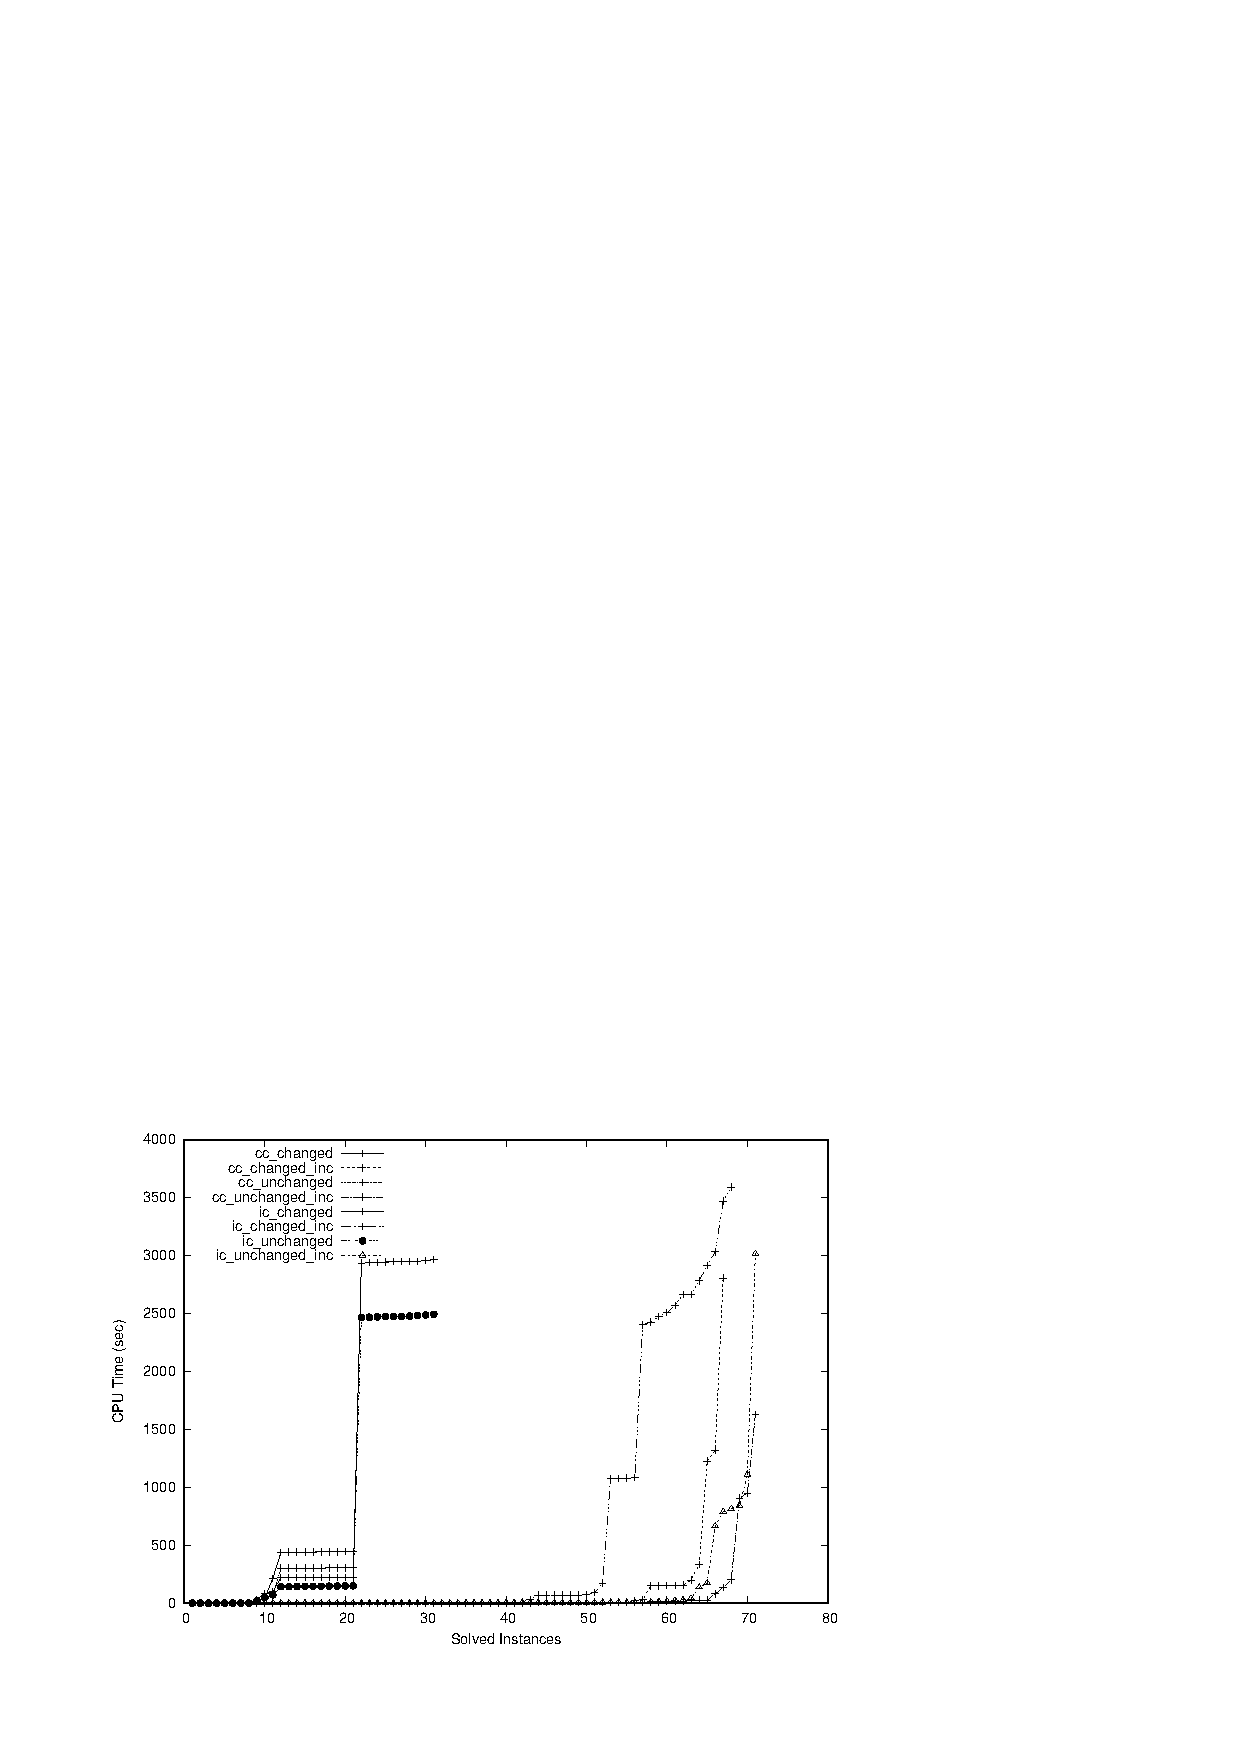
\includegraphics[scale=0.4]{fig/cactus.png}
 \end{figure}

\begin{itemize}
 \item 改良符号化2は,他の符号化と比較して,より多くの問題を高速に解いている.
\end{itemize}\vfill
\end{frame}
%%%%%%%%%%%%%%%%%%%%%%%%%%%%%%%%%%%%%%%%%%%%%%%%%%
%% 辺の数の表
%%%%%%%%%%%%%%%%%%%%%%%%%%%%%%%%%%%%%%%%%%%%%%%%%%
\begin{frame}{実験結果(2/2) : 解けた問題数による比較}
 
\begin{textblock*}{\linewidth}(10pt, 30pt)
\begin{table}[t]
 \begin{tabular}[t]{ccccc}
 \rowcolor[RGB]{0,96,0}
 \color{white} 辺の範囲 & \color{white}問題数 & 
		 \color{white}基本符号化 & \color{white}改良符号化 & \color{white}有向符号化\\
 %%%%%%%%
 \rowcolor[RGB]{230,239,230}
 ~~~~\;\:1 ~ 1,000 & 30 & \alert{30} & \alert{30} & \alert{30} \\
 \rowcolor[RGB]{196,230,196}
 1,001 ~ 4,000 & 20 & \alert{20} & \alert{20} & \alert{20} \\
 \rowcolor[RGB]{230,239,230}
 4,001 ~ 7,000 & 11 & 9 & 10 & \alert{11} \\
 \rowcolor[RGB]{196,230,196}
 ~\:7,001 ~ 10,000 & 8 & 4 & 6 &\alert{7} \\
 \rowcolor[RGB]{230,239,230}
 10,001 ~ 20,000 & 9 & 2 & 5 &\alert{9} \\
 \rowcolor[RGB]{196,230,196}
 20,001 ~ 30,000 & 2 & 1 & \alert{2} & \alert{2} \\
 \rowcolor[RGB]{230,239,230}
 30,001 ~ 40,000 & 1 & 0 & 0 & \alert{1} \\
 \rowcolor[RGB]{196,230,196}
 40,001 ~ 50,000 & 4 & 0 & 2 & \alert{4} \\
 %%%%%%%% 合計
 \noalign{\hrule height 0.5pt}
 \rowcolor[RGB]{230,239,230}
 計 & 85 & 66 & 75 & \alert{84} \\
 
\end{tabular}

\end{table}\vfill

\begin{itemize}
 \item 改良符号化2は,ベンチマーク問題85問中,\textbf{84問}を解いている.
 \item 大規模な問題に対しても改良符号化2は,優位性を示した.
\end{itemize}\vfill
\end{textblock*}
\end{frame}
%%%%%%%%%%%%%%%%%%%%%%%%%%%%%%%%%%%%%%%%%%%%%%%%%%
%% 電気制約 方針
%%%%%%%%%%%%%%%%%%%%%%%%%%%%%%%%%%%%%%%%%%%%%%%%%%
\begin{frame}{電気制約への方針}
 \begin{itemize}
  \item 変電所を定電流源と仮定すると,各配電区間での電流の大きさは\structure{\bf 一定の値}として表される.
  \item 供給経路が決まると,ある配電区間に流れる電流は,その配電区間以下の
		電流の大きさの\alert{\bf 線形和}として表すことができる.
  \item グラフでの直感的な意味は,各連結成分の\structure{\bf 根からの深さ}が大きくなるほど,
		上流での電流は大きくなることを意味する.
  \item 根からの深さを表す変数を導入することで,
		各区間に流れる電流の値を計算することができ,\structure{\bf 電流の電気制約には対応可能}.
		\begin{itemize}
		 \item 実際には配電システム(三相交流)についての特殊な計算が必要.
		\end{itemize}
 \end{itemize}\vfill
 \begin{exampleblock}{例}
  \centering
  %%%%%%%%%%%%%%%%%%%%%%%%%%%%%%%%%%%%%%%%%%%%%%%%%%
% 電気制約の例
%%%%%%%%%%%%%%%%%%%%%%%%%%%%%%%%%%%%%%%%%%%%%%%%%%

\begin{tikzpicture}[scale=0.5]

 % 設定
 \tikzset{node/.style={rectangle, draw=black,fill=white}}

 \definecolor{edge1}{RGB}{191,0,0}
 \definecolor{node1}{RGB}{249,200,200}
 \definecolor{edge3}{RGB}{38,38,134}
 \definecolor{node3}{RGB}{200,200,249}

 % 補助線
 % \draw [help lines,blue] (0,0) grid (20,6);

 % node %
 \node[circle, ultra thick, draw=edge1, fill=node1,minimum size=1cm](1){};
 \node[node, thick, fill=node1, draw=edge1, right=2.5cm of 1] (2){};
 \node[node, thick, fill=node1, draw=edge1, right=3cm of 2] (3){};
 \node[node, thick, fill=node1, draw=edge1, right=2.5cm of 3] (4){};

 % 変電所 %
 \begin{scope}[scale=1.5]
 \draw [ultra thick, draw=edge1] (0,0) circle [radius=0.225cm] node[minimum size=0.5cm](root1){};
 \draw [ultra thick, draw=edge1] (0.225,0)--(0.35,0)--(0.35,0.35);
 \draw [ultra thick, draw=edge1] (-0.225,0)--(-0.35,0)--(-0.35,-0.35);
 \draw [ultra thick, draw=edge1] (0,0.225)--(0,0.35);
 \draw [ultra thick, draw=edge1] (0,-0.225)--(0,-0.35);
 \draw [ultra thick, draw=edge1] [domain=-0.284:-0.159] plot(\x,\x);
 \draw [ultra thick, draw=edge1] [domain=0.159:0.284] plot(\x,\x);
 \draw [ultra thick, draw=edge1] [domain=-0.284:-0.159] plot(\x,-\x);
 \draw [ultra thick, draw=edge1] [domain=0.159:0.284] plot(\x,-\x);
 \end{scope}

 \draw [line width=3.5pt, edge1] (1) -- %
 node[above, font=\Large, label=below:\color{black}{$I_i\colon\quad$30A}]
 {\textbf{$J_i\colon\quad$\!\!60A}}(5,0) -- (2);
 
 \draw [line width=2.5pt, edge1] (2) -- %
 node[above, font=\Large, label=below:\color{black}{20A}] {\textbf{30A}}(11,0) -- (3);

 \draw [line width=1.5pt, edge1] (3) -- %
 node[above, font=\large, label=below:\color{black}{10A}] {\textbf{10A}}(17,0) -- (4);

\end{tikzpicture}

%%%%%%%%%%%%%%%%%%%%%%%%%%%%%%%%%%%%%%%%%%%%%%%%%%%%%%%%%%
%%% Local Variables:
%%% mode: japanese-latex
%%% TeX-master: ``slide''
%%% End:

 \end{exampleblock} \vfill
\end{frame}
%%%%%%%%%%%%%%%%%%%%%%%%%%%%%%%%%%%%%%%%%%%%%%%%%%
%% まとめ
%%%%%%%%%%%%%%%%%%%%%%%%%%%%%%%%%%%%%%%%%%%%%%%%%%
\begin{frame}{まとめ}
 \begin{enumerate}
  \item \structure{\bf 根付き全域森問題を解くASP符号化を新たに1種類考案}
		\begin{itemize}
		 \item 双方向グラフに拡張することで,各ノードの入次数の制約を用いて
			   非閉路制約を簡潔に記述できることを確認した.
		\end{itemize}
  \item \structure{\bf 実用規模の問題,および,より大規模な問題を用いて評価}
		\begin{itemize}
		 \item 新たに考案した改良符号化2は,大規模な問題に対する有効性など,
			   これまでに考案した符号化よりも更によい性能を示した.
		\end{itemize}
  \item \structure{\bf 電気制約の実装への方針}
		\begin{itemize}
		 \item 定電流源の場合では,電流を線形和として表せることを確認した.
		\end{itemize}
 \end{enumerate} \vfill
 \begin{alertblock}{今後の課題}
  \begin{itemize}
   \item \textit{clingo} の組み込みの制約 ~\texttt{\#edge}を用いた非閉路制約の実装.
   \item 三相交流での電流の大きさなどの計算方法の学習.
   \item 電流の制約を含めた符号化の開発.
  \end{itemize}
 \end{alertblock} \vfill
\end{frame}

%###########################################################
%##### 補助スライド ########################################
%###########################################################

%%%% 補助スライド
\appendix
\backupbegin

\begin{frame}{~}
 \centering
 - 補足用 -
\end{frame} 

%%%%%%%%%%%%%%%%%%%%%%%%%%%%%%%%%%%%%%%%%%%%%%%%%%
%% 電気制約
%%%%%%%%%%%%%%%%%%%%%%%%%%%%%%%%%%%%%%%%%%%%%%%%%%
\begin{frame}{補足 : 電気制約}
 \begin{itemize}
  \item \alert{電気制約}は,送電する電流$\cdot$電圧の適正範囲を保証する制約.
  \begin{itemize}
   \item 供給経路の各区間で許容電流を超えない.
   \item 電気抵抗による電圧降下が許容範囲を超えない.
   \item etc.
  \end{itemize}
  \item 電流と電圧が影響し合う\structure{実数ドメイン上の制約}によって表される.
		% \begin{itemize}
		%  		 \item 送電システム上の条件など.
		% \end{itemize}
  \item 実数ドメイン上の制約は,純粋なASPのみで扱うのは\alert{困難}.
		\begin{itemize}
		 \item 緩和問題として,変電所から供給できる家庭の数に上限をつける.
		 \item ASPMT技術により,ASPで得られた解について,
			   背景理論ソルバーと連携して実数ドメイン上の制約を調べる.
		\end{itemize}
 \end{itemize}
\end{frame}

%%%%%%%%%%%%%%%%%%%%%%%%%%%%%%%%%%%%%%%%%%%%%%%%%%
%% 基礎化
%%%%%%%%%%%%%%%%%%%%%%%%%%%%%%%%%%%%%%%%%%%%%%%%%%
\begin{frame}{補足 : ASPシステム}
 
 \vspace{-0.5cm}

 \begin{figure}[htbp]
  \centering
  %%%%%%%%%%%%%%%%%%%%%%%%%%%%%%%%%%%%%%%%%%%%%%%%%%
%% 基礎化の流れの図
%%%%%%%%%%%%%%%%%%%%%%%%%%%%%%%%%%%%%%%%%%%%%%%%%%
\begin{tikzpicture}

 \definecolor{edge}{RGB}{38,38,134}
 \definecolor{node}{RGB}{220,220,249}

 \definecolor{alert_edge}{RGB}{191,0,0}
 \definecolor{alert_node}{RGB}{249,200,200}

 \definecolor{ex_edge}{RGB}{0,96,0}
 \definecolor{ex_node}{RGB}{230,239,230}

 \def\nodespace{2.4cm}

 \tikzset{block/.style={rectangle, thick, draw=edge, fill=node, text width=3cm, 
 text centered, rounded corners, text width=2cm, minimum height=1.5cm}};

 \tikzset{alertblock/.style={rectangle, thick, draw=alert_edge, fill=alert_node, 
 text width=3cm, text centered, rounded corners, text width=1.5cm, minimum height=1.2cm}};

 \node[block](ikkai){一階ASP\\プログラム};

 \node[rectangle,rounded corners, thick, draw=ex_edge, fill=ex_node, 
 right=0.22*\nodespace of ikkai, minimum width=6cm, minimum height=3cm, 
 text centered, label=ASPシステム](sys){};

 \node[block, right=\nodespace of ikkai](meidai){命題ASP\\プログラム};
 \node[block, right=\nodespace of meidai](ASP){解集合};

 \node[right=0.6*\nodespace of ikkai, text width=1.5cm, 
 text centered, text=red, anchor=south](){基礎化\\ソルバー};
 \node[right=0.4*\nodespace of meidai, text width=1.5cm, 
 text centered, text=red, anchor=south](){解集合\\ソルバー};

 
 \foreach \u / \v / \n in {ikkai/meidai,meidai/ASP}
 \draw [thick,->] (\u) to (\v);

\end{tikzpicture}
 \end{figure}

 \vspace{-0.5cm}

 \begin{exampleblock}{}
  \begin{enumerate}
   \item 一階ASPプログラムを基礎化ソルバーによって,
		 命題ASPプログラムに\alert{基礎化}する.
   \item 命題ASPプログラムについて,SAT技術を応用した解集合ソルバーが解集合を探索する.
  \end{enumerate}
 \end{exampleblock}

\end{frame}
%%%%%%%%%%%%%%%%%%%%%%%%%%%%%%%%%%%%%%%%%%%%%%%%%%
%% ASPの構文
%%%%%%%%%%%%%%%%%%%%%%%%%%%%%%%%%%%%%%%%%%%%%%%%%%
\begin{frame}{ASPの構文}
  \begin{alertblock}{}\centering
    ASPの言語は論理プログラムをベースとしている~\footnotemark.
  \end{alertblock}
  \begin{itemize}
  \item \structure{\bf 論理プログラム}とは,以下の\structure{\bf ルール}の有限集合である.
    \begin{center}
      \begin{minipage}[c]{0.7\textwidth}
        \begin{block}{}\centering
          $a_0$\quad\code{:-}\quad$a_1$\code{,}\ldots\code{,}$a_m$\code{,}
          \ \code{not}~$a_{m+1}$\code{,}\ldots\code{,} \code{not}~$a_n$\code{.}
        \end{block}        
      \end{minipage}
   \end{center}\vfill
    $0 \leq m \leq n$ であり,各 $a_i$ はアトム,
    \code{not}は\structure{\bf デフォルトの否定},\\
    ``\code{,}''は連言(AND)を表す.``\code{:-}''の左辺を\structure{\bf ヘッド},
		右辺を\structure{\bf ボディ}と呼ぶ.
  \item \alert{\bf 直感的な意味}は,
    「$a_1,\ldots,a_m$がすべて成り立ち,
    $a_{m+1},\ldots,a_n$のそれぞれが成り立たないならば,
    $a_0$が成り立つ」である.
  \item ボディが空のルールを\structure{\bf ファクト}と呼び,``\code{:-}''は省略できる.
  \item ヘッドが空のルールを\structure{\bf 一貫性制約}と呼ぶ.例えば,\hspace{-1ex}
    ``\code{:-} $a_1$\code{,} \code{not}~$a_{2}$''は,
    「$a_1$が成り立つならば,$a_2$が成り立つ」を意味する.
  \end{itemize}
  \footnotetext{本発表では標準論理プログラムを単に論理プログラムと呼ぶ.}
\end{frame}
%%%%%%%%%%%%%%%%%%%%%%%%%%%%%%%%%%%%%%%%%%%%%%%%%%
%% ASPの拡張構文
%%%%%%%%%%%%%%%%%%%%%%%%%%%%%%%%%%%%%%%%%%%%%%%%%%
\begin{frame}{ASPの拡張構文}
\begin{alertblock}{}\centering
  組合せ問題を解くための便利な構文が用意されている.
\end{alertblock}
\begin{itemize}
 \item \structure{\bf 選択子}
   \begin{center}
     \code{\{}$a_1$\code{;}\ldots\code{;}$a_n$\code{\}}
   \end{center}
   アトム集合 $\{a_1,\dots,a_n\}$
   の任意の部分集合が成り立つことを意味する.
 \item \structure{\bf 個数制約}
   \begin{center}
     $lb$\ \code{\{}$a_1$\code{;}\ldots\code{;}$a_n$\code{\}}\ $ub$
   \end{center}
   $a_1,\dots,a_n$ のうち,
   $lb$個以上,$ub$個以下が成り立つことを意味する.
 \item \structure{\bf 重み付き個数制約}
   \begin{center}
     $lb$ \code{\#sum\{} $w_1$\code{:}$a_1$\code{;}\ldots\code{;}$w_n$\code{:}$a_n$ \code{\}} $ub$
   \end{center}
   $a_1,\dots,a_n$のうち,
   成り立つアトムの重み和が$lb$以上,$ub$以下になることを意味する.
\end{itemize}
\end{frame}
%%%%%%%%%%%%%%%%%%%%%%%%%%%%%%%%%%%%%%%%%%%%%%%%%%
%% 改良符号化 (到達可能性)
%%%%%%%%%%%%%%%%%%%%%%%%%%%%%%%%%%%%%%%%%%%%%%%%%%
\begin{frame}[fragile]{改良符号化: 到達可能性}
\begin{exampleblock}{}\small
\begin{lstlisting}
(1) { inForest(X,Y) } :- edge(X,Y).
\end{lstlisting}
\end{exampleblock}
\begin{itemize}
 \item (1) 各辺\code{(X,Y)について},根付き全域森に含まれること意味する \\
	  アトム\code{inForest(X,Y)}を導入する.
\end{itemize}
\begin{exampleblock}{}\small
\begin{lstlisting}
(2) reached(R,R) :- root(R).
(3) reached(X,R) :- reached(Y,R), inForest(Y,X).
(4) reached(X,R) :- reached(Y,R), inForest(X,Y).
\end{lstlisting}
\end{exampleblock}
\vfill
\begin{itemize}
\item アトム\code{reached(X,R)}は,ノード\code{X}が根ノード\code{R}から到達可能であることを意味する.
%\item (2) 各根ノード\code{R}について,自分自身から到達可能であることを表す.
\item (3) ノード\code{Y}が根ノード\code{R}から到達可能かつ,辺\code{(Y,X)}が根付き全域森に含まれるならば,
	  ノード\code{X}も同じ根ノード\code{R}から到達可能であることを表す.
\end{itemize}
\end{frame}
%%%%%%%%%%%%%%%%%%%%%%%%%%%%%%%%%%%%%%%%%%%%%%%%%%
%% 改良符号化 (根付き連結制約)
%%%%%%%%%%%%%%%%%%%%%%%%%%%%%%%%%%%%%%%%%%%%%%%%%%
\begin{frame}[fragile]{改良符号化: 根付き連結制約}
\begin{exampleblock}{}\small
\begin{lstlisting}
(5) :- node(X), not 1 { reached(X,R) } 1.
\end{lstlisting}
\end{exampleblock}
\vfill
\begin{itemize}
\item (5) 各ノード\code{X}について,ちょうど1つの根からのみ到達可能であることを意味する.
\end{itemize}
\end{frame}
%%%%%%%%%%%%%%%%%%%%%%%%%%%%%%%%%%%%%%%%%%%%%%%%%%
%% 改良符号化 (非閉路制約)
%%%%%%%%%%%%%%%%%%%%%%%%%%%%%%%%%%%%%%%%%%%%%%%%%%
\begin{frame}[fragile]{改良符号化: 非閉路制約}
\begin{minipage}[c]{1.01\textwidth}
\begin{exampleblock}{}\small
\begin{lstlisting}
(6) :- root(R),
       not 1 #sum{ 1,X:reached(X,R) ;
                  -1,X,Y:inForest(X,Y),reached(X,R),reached(Y,R)
                 } 1.
\end{lstlisting}
\end{exampleblock}
\end{minipage}
\vfill
\begin{itemize}
\item (6) 各連結成分の\structure{\bf ノード数と辺数の差が1}になることを意味する.
\item 各連結成分が\structure{\bf 木の性質}を満たすことにより,サイクルを持たない
	  ことを保証する.
\end{itemize}
\end{frame}
%%%%%%%%%%%%%%%%%%%%%%%%%%%%%%%%%%%%%%%%%%%%%%%%%%
%% ルール数の比較
%%%%%%%%%%%%%%%%%%%%%%%%%%%%%%%%%%%%%%%%%%%%%%%%%%
\begin{frame}{基礎化後のルール数}
  \begin{itemize}
  \item グラフのノード数を$|V|$,根ノードの数を$|R|$とする.
  \end{itemize}
  \begin{table}[t]
    \centering
    %%%%%%%%%%%%%%%%%%%%%%%%%%%%%%%%%%%%%%%%%%%%%%%%%%%%%%%%%%%%%%%%
\chapter{ハミルトン閉路問題および関連問題のASP符号化}\label{chap:proposal}
%%%%%%%%%%%%%%%%%%%%%%%%%%%%%%%%%%%%%%%%%%%%%%%%%%%%%%%%%%%%%%%% 

%%%%
\begin{figure}[h]
  \centering
  \thicklines
  \setlength{\unitlength}{1.2pt}
  \small\footnotesize\scriptsize
  \begin{picture}(280,57)(4,-10)
    \put(  0, 20){\dashbox(50,24){\shortstack{HCP問題\\インスタンス}}}
    \put( 60, 20){\framebox(50,24){変換器}}
    \put(120, 20){\dashbox(50,24){\shortstack{ASPファクト}}}
    \put(120,-10){\dashbox(50,24){\shortstack{ASP符号化\\(論理プログラム)}}}
    \put(180, 20){\framebox(50,24){ASPシステム}}
    \put(240, 20){\dashbox(50,24){\shortstack{HCP問題\\の解}}}
    \put( 50, 32){\vector(1,0){10}}
    \put(110, 32){\vector(1,0){10}}
    \put(170, 32){\vector(1,0){10}}
    \put(230, 32){\vector(1,0){10}}
    \put(170, +2){\line(1,0){4}}
    \put(174, +2){\line(0,1){30}}
  \end{picture}  
\caption{ASP を用いたハミルトン閉路問題(HCP)の解法}
\label{fig:arch}
\end{figure}
%%%%

%\begin{figure}[tbp]
\tikz{
  %1ノード目
  \path[draw=black, fill=blue!20, rounded corners=5pt]%線の設定
  node[at={(0.75,0.75)}] {問題}%文字を入れる
  (0,0) --(1.5,0) --(1.5,1.5) --(0,1.5) --cycle;%外周
  %2ノード目
  \path[draw=black, fill=blue!20, rounded corners=5pt, shift={(3,0)}]
  node[at={(0.75,0.75)}] {
    \begin{tabular}{c}
      ASP\\
      ファクト
    \end{tabular}
  }
  (0,0) --(1.5,0) --(1.5,1.5) --(0,1.5) --cycle;
  %3ノード目文字が複数行
  \path[draw=black, fill=green!20, rounded corners=5pt, shift={(6,0)}]
  node[at={(0.75,0.75)}] {
    \begin{tabular}{c}
      ASP\\
      システム
    \end{tabular}
  }
  (0,0) --(1.5,0) --(1.5,1.5) --(0,1.5) --cycle;
  %4ノード目文字が複数行
  \path[draw=black, fill=blue!20, rounded corners=5pt, shift={(9,0)}]
  node[at={(0.75,0.75)}] {解集合}
  (0,0) --(1.5,0) --(1.5,1.5) --(0,1.5) --cycle;
  %5ノード目文字が複数行
  \path[draw=black, fill=red!20, rounded corners=5pt, shift={(3,-3)}]
  node[at={(0.75,0.75)}] {
    \begin{tabular}{c}
      ASP\\
      符号化
    \end{tabular}
  }
  (0,0) --(1.5,0) --(1.5,1.5) --(0,1.5) --cycle;
  \draw[arrows=->] (1.5,0.75) --(3.0,0.75);
  \draw[arrows=->,shift={(3,0)}] (1.5,0.75) --(3.0,0.75);
  \draw[arrows=->,shift={(6,0)}] (1.5,0.75) --(3.0,0.75);
  \draw[arrows=->] (4.5,-2.25) --(6.0,0.5);
}
\caption{ASPを用いた解法}
\label{aspmethod}
\end{figure}


ASP を用いたハミルトン閉路問題および関連問題の解法について述べる.
図~\ref{fig:arch}に,解法の流れを示す.
与えられたハミルトン閉路問題は ASP ファクトに変換され,
ハミルトン閉路問題を解く ASP 符号化と結合され,
ASP システムによって解が計算される.
本論文では,ASP システムとして{\clingo}を用いる.

%%%%%%%%%%%%%%%%%%%%%%%%%%%%%%%%%%%%%%%%%%%%%%%%%%%%%%%%%%%%%%%%%%%%%%%
\section{ASPファクト形式}
%%%%%%%%%%%%%%%%%%%%%%%%%%%%%%%%%%%%%%%%%%%%%%%%%%%%%%%%%%%%%%%%%%%%%%%

%%%%%%%%%%%%%%%%%%%%%%%%%%%%%%
\begin{figure}[t]
\begin{center}
\begin{tikzpicture}
  %ノード1  
  \draw(4,2) circle (0.5)
  node[at={(4.1,2.1)}] {
    \begin{tabular}{c}
      1
    \end{tabular}
  };
  %ノード2  
  \draw(4,0) circle (0.5)
  node[at={(4.1,0.1)}] {
    \begin{tabular}{c}
      2
    \end{tabular}
  };
  %ノード3  
  \draw(6,2) circle (0.5)
  node[at={(6.1,2.1)}] {
    \begin{tabular}{c}
      3
    \end{tabular}
  };
  %ノード4  
  \draw(6,0) circle (0.5)
  node[at={(6.1,0.1)}] {
    \begin{tabular}{c}
      4
    \end{tabular}
  };
  %ノード5  
  \draw(8,2) circle (0.5)
  node[at={(8.1,2.1)}] {
    \begin{tabular}{c}
      5
    \end{tabular}
  };
  %ノード6  
  \draw(8,0) circle (0.5)
  node[at={(8.1,0.1)}] {
    \begin{tabular}{c}
      6
    \end{tabular}
  };
\draw(4,0.5) --(4,1.5);
\draw(6,0.5) --(6,1.5);
\draw(8,0.5) --(8,1.5);
\draw(4.5,0) --(5.5,0);
\draw(4.5,2) --(5.5,2);
\draw(6.5,0) --(7.5,0);
\draw(6.5,2) --(7.5,2);
\end{tikzpicture}

\caption{入力となる重み付き無向グラフの例}
\label{graphexample}
\end{center}
\end{figure}
%%%%%%%%%%%%%%%%%%%%%%%%%%%%%%

%%%%%%%%%%%%%%%%%%%%%%%%%%%%%%
\lstinputlisting[float=t,caption={%
図~\ref{graphexample}のASPファクト表現},%
captionpos=b,frame=single,label=code:graph_example.lp,%
numbers=none,%
breaklines=true,%
columns=fullflexible,keepspaces=true,%
basicstyle=\ttfamily\scriptsize]{code/graph_example.lp}
%%%%%%%%%%%%%%%%%%%%%%%%%%%%%%


本節では,最短ハミルトン閉路問題の例にとって,
入力となる重み付き無向グラフ(図~\ref{graphexample})の
ASP ファクト形式について説明する.
%
このグラフは,頂点数が6,辺の数が7であり,辺に付けられた値は距離を表す.
コード~\ref{code:graph_example.lp}に,ASPファクト形式を示す.
%
アトム\code{node/1}は頂点,\code{edge/2}は辺,\code{cost/3}は距離を表す.
例えば,\code{cost(1,2,3)}は,辺\code{edge(1,2)}の距離が3であることを
表している.

%%%%%%%%%%%%%%%%%%%%%%%%%%%%%%%%%%%%%%%%%%%%%%%%%%%%%%%%%%%%%%%%%%%%%%%
\section{ハミルトン閉路問題の ASP 符号化}\label{hamiltonianasp}
%%%%%%%%%%%%%%%%%%%%%%%%%%%%%%%%%%%%%%%%%%%%%%%%%%%%%%%%%%%%%%%%%%%%%%%

ハミルトン閉路問題は,与えられたグラフの全頂点をちょうど一度ずつ通る閉
路(ハミルトン閉路)が存在するかどうかを判定する問題である.
$G=(V,E)$にハミルトン閉路が存在する必要十分条件は,
以下の2つの制約を満たす部分グラフ$G'=(V,E')$が存在することである.

\begin{itemize}
\item $G'$の各頂点の次数が2 (次数制約)
\item $G'$が連結である (連結制約)
\end{itemize}

本論文では,前者を\textbf{次数制約},後者を\textbf{連結制約}と呼ぶ.
ハミルトン路問題は,ハミルトン閉路問題から始点と終点が一致するという閉
路の条件を取り除いたものである.
ハミルトン路問題では,次数制約は以下のように変わる.

\begin{itemize}
\item 始点と終点の次数が1,他の頂点の次数が2
\end{itemize}

以下では,ハミルトン閉路問題に対する3つの ASP 符号化
\textsf{undirected},\textsf{directed},\textsf{acyclicity}
を提案する.

%%%%%%%%%%%%%%%%%%%%%%%%%%%%%%%%%%%%%%%%%%%%%%%%%%%%%%%%%%%%%%%%%%%%%%%
\subsection{\textsf{undirected}符号化}
%%%%%%%%%%%%%%%%%%%%%%%%%%%%%%%%%%%%%%%%%%%%%%%%%%%%%%%%%%%%%%%%%%%%%%%

%%%%%%%%%%%%%%%%%%%%%%%%%%%%%%
\lstinputlisting[float=t,caption={%
\textsf{undirected}符号化},%
captionpos=b,frame=single,label=code:hamilton1.lp,%
numbers=left,%
breaklines=true,%
columns=fullflexible,keepspaces=true,%
basicstyle=\ttfamily\footnotesize]{code/hamilton1.lp}
%%%%%%%%%%%%%%%%%%%%%%%%%%%%%%

\textsf{undirected}符号化は,ハミルトン閉路問題の次数制約と連結制約を,
ASP の一貫性制約で表した基本的な符号化である.
コード~\ref{code:hamilton1.lp}に,\textsf{undirected}符号化を示す.
この符号化は,ハミルトン閉路問題とハミルトン路問題の両方に対応している.
符号化中の\code{s}は始点の頂点番号,\code{t}は終点の頂点番号を表し,こ
れらは実行時に与えられる.
ここでは,ハミルトン閉路問題(\code{s}=\code{t})の場合について説明する.

\begin{itemize}
\item 1行目のルールは,各辺\code{edge(X,Y)}に対して,その辺がハミルト
  ン閉路に含まれるかどうかを意味するアトム\code{in(X,Y)}を選択子を用い
  て導入している.
\item 次数制約は3行目のルールで表される.このルールは,
  各頂点\code{node(X)}に対して,その次数の和が2に等しいことを個数制約
  を使って表している.
\item 連結制約は11行目のルールで表される.
ある頂点\code{X}が始点\code{s}から到達可能であることを意味する補助アト
ム\code{reached(X)}を導入する.
8行目のルールは,始点\code{s}が到達可能あることを表している.
9行目のルールは,各辺\code{X}--\code{Y}に対して,その辺がハミルトン閉
路に含まれ(\code{in(X,Y)}),かつ,頂点\code{X}が始点から到
達可能であれば(\code{reached(X)}),\code{Y}も到達可能であることを表している.
10行目は9行目と同様であるが,辺\code{Y}--\code{X}の場合を表している.
11行目のルールは,各頂点\code{node(X)}が始点から到達可能でなければな
らないことを一貫性制約を使って表している.
\end{itemize}

%%%%%%%%%%%%%%%%%%%%%%%%%%%%%%%%%%%%%%%%%%%%%%%%%%%%%%%%%%%%%%%%%%%%%%%
\subsection{\textsf{directed}符号化}
%%%%%%%%%%%%%%%%%%%%%%%%%%%%%%%%%%%%%%%%%%%%%%%%%%%%%%%%%%%%%%%%%%%%%%%

%%%%%%%%%%%%%%%%%%%%%%%%%%%%%%
\lstinputlisting[float=t,caption={%
\textsf{directed}符号化},%
captionpos=b,frame=single,label=code:hamilton2.lp,%
numbers=left,%
breaklines=true,%
columns=fullflexible,keepspaces=true,%
basicstyle=\ttfamily\footnotesize]{code/hamilton2.lp}
%%%%%%%%%%%%%%%%%%%%%%%%%%%%%%

\textsf{directed}符号化は,\textsf{undirected}符号化をベースに,
与えられた無向グラフの各辺$u-v$に対して,2つの弧$u\rightarrow v$と
$v\rightarrow u$を対応させることで有向グラフ化して解く符号化である.
コード~\ref{code:hamilton2.lp}に,\textsf{directed}符号化を示す.
前節と同様に,ハミルトン閉路問題(\code{s}=\code{t})の場合について説明する.

\begin{itemize}
\item 1行目では,無向グラフの有向グラフ化を行う.
  与えられた無向グラフの各辺\code{edge(X,Y)}に対して,
  2つの弧\code{edge(X,Y)},\code{edge(Y,X)}を導入した.
\item 2行目のルールは,各弧\code{edge(X,Y)}に対して,その弧がハミルト
  ン閉路に含まれるかどうかを意味するアトム\code{in(X,Y)}を選択子を用い
  て導入している.
\item 次数制約は4,5行目のルールで表される.
  4行目では,各頂点\code{node(X)}に対して,
  その出次数が1に等しいことを個数制約を使って表している.
  5行目では,入次数について4行目と同様の制約を表す.
\item 連結制約は15行目のルールで表される.
  ある頂点\code{X}が始点\code{s}から到達可能であることを意味する
  補助アトム\code{reached(X)}を導入する.
  13行目のルールは,始点\code{s}が到達可能あることを表している.
  14行目のルールは,各弧\code{X}--\code{Y}に対して,その弧がハミルトン閉路
  に含まれ(\code{in(X,Y)}),かつ,頂点\code{X}が始点から
  到達可能であれば(\code{reached(X)}),\code{Y}も到達可能であることを表している.
  15行目のルールは,各頂点\code{node(X)}が始点から到達可能でなければ
  ならないことを一貫性制約を使って表している.
\item 18行目のルールは,解についての対称性を除去する.
  与えられた無向グラフ上の各ハミルトン閉路に対して,
  それを変換した有向グラフ上のハミルトン閉路は対称な2つが存在する.
  これによる解の重複を防ぐために,18行目のルールは,各弧\code{s}--\code{X},
  \code{Y}--\code{s}がハミルトン閉路に含まれるならば(\code{in(s,X),in(Y,s)}),
  \code{X < Y}でなければならないことを,一貫性制約を用いて表している
\end{itemize}

%%%%%%%%%%%%%%%%%%%%%%%%%%%%%%%%%%%%%%%%%%%%%%%%%%%%%%%%%%%%%%%%%%%%%%%
\subsection{\textsf{acyclicity}符号化}
%%%%%%%%%%%%%%%%%%%%%%%%%%%%%%%%%%%%%%%%%%%%%%%%%%%%%%%%%%%%%%%%%%%%%%%

%%%%%%%%%%%%%%%%%%%%%%%%%%%%%%
\lstinputlisting[float=t,caption={%
\textsf{acyclicity}符号化},%
captionpos=b,frame=single,label=code:hamilton3.lp,%
numbers=left,%
breaklines=true,%
columns=fullflexible,keepspaces=true,%
basicstyle=\ttfamily\footnotesize]{code/hamilton3.lp}
%%%%%%%%%%%%%%%%%%%%%%%%%%%%%%

\textsf{acyclicity}符号化は,\textsf{directed}符号化をベースに,
連結の制約に代わる部分閉路禁止制約を組込み非閉路制約で表現した符号化である.
コード~\ref{code:hamilton3.lp}に,\textsf{acyclicity}符号化を示す.
前節と同様に,ハミルトン閉路問題(\code{s}=\code{t})の場合について説明する.

\begin{itemize}
\item 1行目では,無向グラフの有向グラフ化を行う.
  与えられた無向グラフの各辺\code{edge(X,Y)}に対して,
  2つの弧\code{edge(X,Y)},\code{edge(Y,X)}を導入した.
\item 2行目のルールは,各弧\code{edge(X,Y)}に対して,その弧がハミルト
  ン閉路に含まれるかどうかを意味するアトム\code{in(X,Y)}を選択子を用い
  て導入している.
\item 次数制約は4,5行目のルールで表される.
  4行目では,各頂点\code{node(X)}に対して,
  その出次数が1に等しいことを個数制約を使って表している.
  5行目では,入次数について4行目と同様の制約を表す.
\item 部分閉路禁止制約は14行目のルールで表される.
  このルールは,始点でない各頂点\code{X},\code{Y}について,
  弧\code{X}--\code{Y}がハミルトン閉路に含まれるならば(\code{in(X,Y)}),
  そのような弧の集合をもつグラフが閉路をもたないことを,\code{#edge}宣言を用いて表す.
  ようするに,始点(終点)を含まないような閉路を禁止している.
\item 17行目のルールは,解についての対称性を除去する.
  与えられた無向グラフ上の各ハミルトン閉路に対して,
  それを変換した有向グラフ上のハミルトン閉路は対称な2つが存在する.
  これによる解の重複を防ぐために,17行目のルールは,各弧\code{s}--\code{X},
  \code{Y}--\code{s}がハミルトン閉路に含まれるならば(\code{in(s,X),in(Y,s)}),
  \code{X < Y}でなければならないことを,一貫性制約を用いて表している
\end{itemize}

%%%%%%%%%%%%%%%%%%%%%%%%%%%%%%%%%%%%%%%%%%%%%%%%%%%%%%%%%%%%%%%%%%%%%%% 
\section{最短ハミルトン閉路問題のASP符号化}\label{minexpl}
%%%%%%%%%%%%%%%%%%%%%%%%%%%%%%%%%%%%%%%%%%%%%%%%%%%%%%%%%%%%%%%%%%%%%%% 

%% %%%%%%%%%%%%%%%%%%%%%%%%%%%%%%
%% \lstinputlisting[caption =  最適化,label = minimize]{code/obj_minimize.lp}
%% %%%%%%%%%%%%%%%%%%%%%%%%%%%%%%

%%%%%%%%%%%%%%%%%%%%%%%%%%%%%%
\lstinputlisting[float=t,caption={%
最小化},%
captionpos=b,frame=single,label=code:obj_minimize.lp,%
numbers=left,%
breaklines=true,%
columns=fullflexible,keepspaces=true,%
basicstyle=\ttfamily\footnotesize]{code/obj_minimize.lp}
%%%%%%%%%%%%%%%%%%%%%%%%%%%%%%

最短ハミルトン閉路問題の目的関数は,
ハミルトン閉路を構成する各辺の距離の総和である.
コード\ref{code:obj_minimize.lp}は,
その目的関数の最小化を表す.
このコードは,各辺\code{edge(X,Y)}に対して,その辺がハミルトン閉路に
含まれ(\code{in(X,Y)}),その距離が\code{C}である時に(\code{cost(X,Y,C)}),
\code{C}の総和の最小化を,最小化関数を用いて表している.
.
%%%%%%%%%%%%%%%%%%%%%%%%%%%%%%
\lstinputlisting[float=t,caption={%
重み付き無向グラフの有向グラフ化},%
captionpos=b,frame=single,label=code:cost_both.lp,%
numbers=left,%
breaklines=true,%
columns=fullflexible,keepspaces=true,%
basicstyle=\ttfamily\footnotesize]{code/cost_both.lp}
%%%%%%%%%%%%%%%%%%%%%%%%%%%%%%

符号化directed,acyclicityについては,
与えられた無向グラフの各辺\code{edge(X,Y)}に対して,
2つの弧\code{edge(X,Y)},\code{edge(Y,X)}を導入した.
各辺の距離もこれに対応させるために,コード\ref{code:cost_both.lp}
を追加した.
このルールは,各辺\code{X}--\code{Y}の距離を表す\code{cost(X,Y,C)}について,
\code{cost(Y,X,C)}を導入する.
これにより,与えられた無向グラフの各辺\code{edge(X,Y)}の重み\code{C}が
2つの弧\code{edge(X,Y)},\code{edge(Y,X)}にも付与された.

%%%%%%%%%%%%%%%%%%%%%%%%%%%%%%%%%%%%%%%%%%%%%%%%%%%%%%%%%%%%%%%%%%%%%%% 
\section{コスト制約付きハミルトン閉路のASP符号化}
%%%%%%%%%%%%%%%%%%%%%%%%%%%%%%%%%%%%%%%%%%%%%%%%%%%%%%%%%%%%%%%%%%%%%%% 

%%%%%%%%%%%%%%%%%%%%%%%%%%%%%%
\lstinputlisting[float=t,caption={%
コスト制約},%
captionpos=b,frame=single,label=code:cost_constraint.lp,%
numbers=left,%
breaklines=true,%
columns=fullflexible,keepspaces=true,%
basicstyle=\ttfamily\footnotesize]{code/cost_constraint.lp}
%%%%%%%%%%%%%%%%%%%%%%%%%%%%%%

コスト制約付きハミルトン閉路問題は
ハミルトン閉路問題に,距離の総和が所与の閾値以下 (または以上) であること
を制約条件として付加した問題である.
コード\ref{code:const_constraing.lp}のルールは,その制約を表す.
ルール中の\code{c}は閾値を表し,これは実行時に与えられる.
このルールは,各辺\code{edge(X,Y)}に対して,その辺がハミルトン閉路に
含まれ(\code{in(X,Y)}),その距離が\code{C}である時に(\code{cost(X,Y,C)}),
\code{C}の総和が\code{c}以下でなければならないことを,
一貫性制約と重み付き個数制約を用いて表す.

また,\ref{minexpl}と同様に,
符号化directed,acyclicityについては,
アトム\code{cost}についても有向グラフ化に
対応させるためにコード\ref{code:cost_both.lp}を追加した.
%%%%%%%%%%%%%%%%%%%%%%%%%%%%%%%%%%%%%%%%%%%%%%%%%%%%%%%%%%%%%%%%%%%%%%%

%%% Local Variables:
%%% mode: latex
%%% TeX-master: "paper"
%%% End:

  \end{table}
\end{frame}

%%%%%%%%%%%%%%%%%%%%%%%%%%%%%%%%%%%%%%%%%%%%%%%%%%
%% ASPのコード
%%%%%%%%%%%%%%%%%%%%%%%%%%%%%%%%%%%%%%%%%%%%%%%%%%
\begin{frame}[fragile]{補足 : 根付き全域森 基本符号化}
%%%%%%%%%%%%%%%%%%%%%%%%%%%%%%%%% 
\lstinputlisting[frame=single,label=code:roop,%
xleftmargin=1zw,%
xrightmargin=1zw,%
numbersep=5pt,%
numbers=left,%
breaklines=true,%
columns=fullflexible,keepspaces=true,%
basicstyle=\ttfamily\scriptsize]{code/srf1.lp}
%%%%%%%%%%%%%%%%%%%%%%%%%%%%%%%%%
\end{frame}

\begin{frame}[fragile]{補足 : 遷移問題 シングルショット符号化}

\begin{multicols*}{2}
%%%%%%%%%%%%%%%%%%%%%%%%%%%%%%%%% 
\lstinputlisting[frame=single,label=code:roop,%
xleftmargin=1zw,%
xrightmargin=1zw,%
numbersep=5pt,%
numbers=left,%
breaklines=true,%
columns=fullflexible,keepspaces=true,%
basicstyle=\ttfamily\tiny]{code/trans-const.lp}
%%%%%%%%%%%%%%%%%%%%%%%%%%%%%%%%%
\end{multicols*}
\end{frame}

\begin{frame}[fragile]{補足 : 遷移問題 マルチショット符号化}
\begin{multicols*}{2}
%%%%%%%%%%%%%%%%%%%%%%%%%%%%%%%%%
\lstinputlisting[frame=single,label=code:incmode,% 
xleftmargin=1zw,%
xrightmargin=1zw,%
numbersep=5pt,%
numbers=left,%
breaklines=true,%
columns=fullflexible,keepspaces=true,%
basicstyle=\ttfamily\tiny]{code/dnet-trans.lp}
%%%%%%%%%%%%%%%%%%%%%%%%%%%%%%%%% 
\end{multicols*}
\end{frame}

\backupend


\end{document}
%%% Local Variables:
%%% mode: japanese-latex
%%% TeX-master: t
%%% End:
